% Session 09 – Mid-Course Quiz and Assessment Review
% Deep Learning Course – IIIT Dharwad
% Instructors: Prof. S R M Prasanna & Dr. Sunil Saumya

\documentclass[12pt,a4paper]{article}
\usepackage{amsmath,amsthm,amssymb,mathtools}
\usepackage{tikz}
\usetikzlibrary{arrows.meta,positioning,shapes.geometric,calc,fit,backgrounds}
\usepackage{graphicx}
\usepackage{booktabs,tabularx,multirow}
\usepackage[ruled,vlined,linesnumbered]{algorithm2e}
\usepackage[most]{tcolorbox}
\usepackage{hyperref}
\usepackage[capitalize,noabbrev]{cleveref}
\usepackage[margin=1in]{geometry}
\usepackage{fancyhdr}
\usepackage{enumitem}
\usepackage{xcolor}

%------------------------------------------------------------------
% tcolorbox environments
%------------------------------------------------------------------
\newtcolorbox{keyinsight}[1][]{colback=blue!5!white,colframe=blue!75!black,fonttitle=\bfseries,title=Key Insight,#1}
\newtcolorbox{example}[1][]{colback=green!5!white,colframe=green!75!black,fonttitle=\bfseries,title=Example,#1}
\newtcolorbox{warningbox}[1][]{colback=red!5!white,colframe=red!75!black,fonttitle=\bfseries,title=Warning,#1}

%------------------------------------------------------------------
% amsthm environments
%------------------------------------------------------------------
\newtheorem{theorem}{Theorem}[section]
\newtheorem{lemma}[theorem]{Lemma}
\newtheorem{definition}{Definition}[section]
\newtheorem{remark}{Remark}[section]

%------------------------------------------------------------------
% Header / footer
%------------------------------------------------------------------
\pagestyle{fancy}
\fancyhf{}
\rhead{Deep Learning -- Session 09}
\lhead{IIIT Dharwad}
\cfoot{\thepage}

%------------------------------------------------------------------
% Convenience macros
%------------------------------------------------------------------
\newcommand{\R}{\mathbb{R}}
\newcommand{\loss}{\mathcal{L}}
\newcommand{\sigmoid}{\sigma}

%------------------------------------------------------------------
\begin{document}
%------------------------------------------------------------------

%==================================================================
% TITLE PAGE
%==================================================================
\begin{titlepage}
  \centering
  \vspace*{2cm}
  {\LARGE\bfseries Deep Learning -- Course Notes\par}
  \vspace{0.5cm}
  {\large IIIT Dharwad -- M.Tech / PhD Programme\par}
  \vspace{1.5cm}
  \rule{\linewidth}{0.4pt}\\[0.4cm]
  {\Huge\bfseries Session 09\par}
  \vspace{0.3cm}
  {\Large Mid-Course Quiz, Assessment Review,\\[4pt]
          and Foundations Consolidation\par}
  \rule{\linewidth}{0.4pt}\\[1.5cm]
  \begin{tabular}{ll}
    \textbf{Session number} & 09 \\[4pt]
    \textbf{Topic}          & Mid-course LMS quiz; post-quiz discussion \\[4pt]
    \textbf{Instructors}    & Prof.\ S R M Prasanna \& Dr.\ Sunil Saumya \\[4pt]
    \textbf{Teaching Asst.} & Vial (quiz coordinator) \\[4pt]
    \textbf{Slide deck}     & \texttt{05-PyTorchDL-NNmodule} \\[4pt]
    \textbf{Duration}       & $\approx 75$ minutes \\[4pt]
    \textbf{Date}           & Cohort 2, Academic Year 2025--26 \\
  \end{tabular}
  \vfill
  {\small These notes are reconstructed from the session transcript and\\
  visual extraction log (session09\_transcript.vtt).}
\end{titlepage}

%==================================================================
% TABLE OF CONTENTS
%==================================================================
\tableofcontents
\newpage

%==================================================================
\section{Introduction}
\label{sec:intro}
%==================================================================

Session~09 of the Deep Learning course at IIIT Dharwad served a dual
purpose.  The first and primary part consisted of a timed, LMS-based
mid-course quiz covering material from Sessions~01--08.  The second,
shorter part (roughly 15--20 minutes) was a live post-quiz review in
which Prof.\ Prasanna and the students discussed specific questions,
grading concerns, and the conceptual underpinning of incorrect or
disputed answers.

\medskip
\noindent
This document reconstructs the pedagogical content of that session.
It is structured as follows:
\begin{itemize}[leftmargin=1.5cm]
  \item \cref{sec:prereq} -- Prerequisites: a concise review of the
        topics on which the quiz was based.
  \item \cref{sec:quiz_logistics} -- Quiz logistics, format, and
        grading methodology.
  \item \cref{sec:quiz_topics} -- Topic-by-topic summary of the
        assessed concepts.
  \item \cref{sec:post_quiz_review} -- Post-quiz discussion: disputed
        questions, TensorFlow vs.\ PyTorch issue, and instructor
        clarifications.
  \item \cref{sec:vanishing_gradient} -- Deep-dive: vanishing gradient
        problem (the most-discussed quiz topic).
  \item \cref{sec:frameworks} -- PyTorch vs.\ TensorFlow: a comparative
        overview motivated by the quiz.
  \item \cref{sec:conclusion} -- Summary and outlook toward Sessions~10+.
\end{itemize}

\begin{keyinsight}
Session~09 is an \emph{assessment session}.  No new slides were presented
during the quiz period.  The post-quiz discussion, however, surfaced
several important conceptual clarifications about backpropagation,
gradient flow, and the relationship between PyTorch and TensorFlow --
all of which are examined in depth in this document.
\end{keyinsight}

%==================================================================
\section{Prerequisites and Background}
\label{sec:prereq}
%==================================================================

The quiz assessed cumulative knowledge from Sessions~01--08.  The
following subsections provide a concise review of each major building
block.

%------------------------------------------------------------------
\subsection{Perceptron and the Linear Threshold Unit}
\label{ssec:perceptron}
%------------------------------------------------------------------

A perceptron with $n$ inputs $x_1, \ldots, x_n$, weights
$w_1, \ldots, w_n$, and bias $b$ computes

\begin{equation}
  \hat{y} = \text{step}\!\left(\sum_{i=1}^{n} w_i x_i + b\right),
  \qquad
  \text{step}(z) = \begin{cases} 1 & z \geq 0 \\ 0 & z < 0 \end{cases}
  \label{eq:perceptron}
\end{equation}

\noindent
The \emph{perceptron learning rule} updates weights only when a
misclassification occurs:

\begin{equation}
  w_i \leftarrow w_i + \eta \,(y - \hat{y})\, x_i, \qquad
  b    \leftarrow b    + \eta \,(y - \hat{y})
  \label{eq:perceptron_update}
\end{equation}

\noindent
where $\eta > 0$ is the learning rate and $y \in \{0, 1\}$ is the
target.  The perceptron convergence theorem guarantees that, for any
linearly separable dataset, the algorithm terminates in a finite number
of steps.

\begin{definition}[Linear Separability]
\label{def:lin_sep}
A binary dataset $\{(\mathbf{x}_i, y_i)\}$ is \emph{linearly separable}
if there exists a hyperplane $\mathbf{w}^{\top}\mathbf{x} + b = 0$ such
that all samples with $y_i = 1$ lie on one side and all samples with
$y_i = 0$ lie on the other.
\end{definition}

A canonical non-linearly separable problem is XOR:

\begin{equation}
  \text{XOR}(0,0)=0,\quad
  \text{XOR}(0,1)=1,\quad
  \text{XOR}(1,0)=1,\quad
  \text{XOR}(1,1)=0.
  \label{eq:xor}
\end{equation}

\noindent
A single perceptron cannot solve XOR; a two-layer network (MLP) can.

%------------------------------------------------------------------
\subsection{Multi-Layer Perceptron and Forward Pass}
\label{ssec:mlp}
%------------------------------------------------------------------

An MLP with one hidden layer computes:
\begin{align}
  \mathbf{z}^{(1)} &= W^{(1)}\mathbf{x} + \mathbf{b}^{(1)},
    \label{eq:z1} \\
  \mathbf{a}^{(1)} &= f\!\left(\mathbf{z}^{(1)}\right),
    \label{eq:a1} \\
  \mathbf{z}^{(2)} &= W^{(2)}\mathbf{a}^{(1)} + \mathbf{b}^{(2)},
    \label{eq:z2} \\
  \hat{\mathbf{y}} &= g\!\left(\mathbf{z}^{(2)}\right),
    \label{eq:yhat}
\end{align}
where $f$ is a hidden-layer activation function and $g$ is an output
activation (e.g., softmax for classification or identity for regression).

\begin{remark}
\label{rem:matrix_order}
The convention adopted in PyTorch for a \emph{fully-connected} layer is
$\mathbf{z} = W\mathbf{x} + \mathbf{b}$, i.e., the weight matrix
multiplies the input vector from the \emph{left}.  In the post-quiz
review Prof.\ Prasanna noted that a TensorFlow snippet which placed the
input on the left ($\mathtt{tf.matmul}(X, W) + b$) confused several
students because the convention differs from the class exercises.
\end{remark}

%------------------------------------------------------------------
\subsection{Activation Functions}
\label{ssec:activations}
%------------------------------------------------------------------

\cref{tab:activations} summarises the activation functions covered in
Sessions~05--06.

\begin{table}[htbp]
  \centering
  \caption{Activation functions covered in Sessions~05--06.}
  \label{tab:activations}
  \begin{tabular}{lll}
    \toprule
    \textbf{Function} & \textbf{Formula} & \textbf{Range} \\
    \midrule
    Sigmoid   & $\sigma(z)=\dfrac{1}{1+e^{-z}}$            & $(0,1)$ \\[6pt]
    Tanh      & $\tanh(z)=\dfrac{e^z-e^{-z}}{e^z+e^{-z}}$ & $(-1,1)$ \\[6pt]
    ReLU      & $\max(0,z)$                                 & $[0,\infty)$ \\[4pt]
    Leaky ReLU & $\max(\alpha z,\,z),\;\alpha\ll 1$         & $(-\infty,\infty)$ \\[4pt]
    Step      & $\mathbf{1}[z \geq 0]$                      & $\{0,1\}$ \\
    \bottomrule
  \end{tabular}
\end{table}

%------------------------------------------------------------------
\subsection{Loss Functions}
\label{ssec:loss}
%------------------------------------------------------------------

For regression the Mean Squared Error (MSE) loss over $N$ samples is

\begin{equation}
  \loss_{\text{MSE}} = \frac{1}{N}\sum_{i=1}^{N}\bigl(y_i - \hat{y}_i\bigr)^2.
  \label{eq:mse}
\end{equation}

\noindent
For binary classification with the sigmoid output unit:

\begin{equation}
  \loss_{\text{BCE}} = -\frac{1}{N}\sum_{i=1}^{N}
    \Bigl[y_i \log\hat{y}_i + (1-y_i)\log(1-\hat{y}_i)\Bigr].
  \label{eq:bce}
\end{equation}

%------------------------------------------------------------------
\subsection{Backpropagation and the Chain Rule}
\label{ssec:backprop}
%------------------------------------------------------------------

Backpropagation computes $\partial \loss / \partial W^{(\ell)}$ for
each layer $\ell$ using the chain rule:

\begin{equation}
  \frac{\partial \loss}{\partial W^{(\ell)}}
  = \frac{\partial \loss}{\partial \mathbf{z}^{(\ell)}}
    \cdot
    \frac{\partial \mathbf{z}^{(\ell)}}{\partial W^{(\ell)}}.
  \label{eq:chain}
\end{equation}

\noindent
Defining the \emph{error signal} (delta) at layer $\ell$ as
$\boldsymbol{\delta}^{(\ell)} = \partial \loss / \partial
\mathbf{z}^{(\ell)}$, the backward recurrence is

\begin{align}
  \boldsymbol{\delta}^{(L)} &= \nabla_{\hat{\mathbf{y}}}\loss
    \odot g'\!\left(\mathbf{z}^{(L)}\right), \label{eq:delta_L} \\
  \boldsymbol{\delta}^{(\ell)} &=
    \left({W^{(\ell+1)}}^{\!\top}\boldsymbol{\delta}^{(\ell+1)}\right)
    \odot f'\!\left(\mathbf{z}^{(\ell)}\right), \label{eq:delta_l} \\
  \frac{\partial\loss}{\partial W^{(\ell)}} &=
    \boldsymbol{\delta}^{(\ell)}\,{\mathbf{a}^{(\ell-1)}}^{\!\top}, \label{eq:dL_dW}
\end{align}

\noindent
where $\odot$ denotes element-wise multiplication and $L$ is the number
of layers.

%==================================================================
\section{Quiz Logistics and Format}
\label{sec:quiz_logistics}
%==================================================================

%------------------------------------------------------------------
\subsection{Session Timeline}
\label{ssec:timeline}
%------------------------------------------------------------------

\cref{tab:timeline} gives the chronological structure of Session~09 as
reconstructed from the transcript.

\begin{table}[htbp]
  \centering
  \caption{Session~09 timeline.}
  \label{tab:timeline}
  \begin{tabularx}{\linewidth}{llX}
    \toprule
    \textbf{Timestamp} & \textbf{Phase} & \textbf{Activity} \\
    \midrule
    00:01:03 & Pre-quiz   & Students discussing exam logistics
                            (timing, links, LMS access) \\
    00:07:27 & Pre-quiz   & Session greeting; instructor joins; brief
                            mention of CNN as next topic \\
    00:08:30 & Pre-quiz   & Screen sharing started; instructions given \\
    00:22:18 & Quiz       & Quiz announced; LMS interface instructions \\
    00:23:19 & Quiz       & Camera-on requirement enforced \\
    00:24:17 & Quiz       & Quiz opens at 8:00 AM; students begin \\
    00:38:07 & Quiz       & Student raises question~8 (incomplete
                            $x_3 = 0.\!$\ldots value) \\
    00:48:29 & Post-quiz  & Quiz ends; class resumes \\
    00:49:51 & Post-quiz  & Student Q\&A on question~4 (duplicate
                            options A and C) \\
    00:57:59 & Post-quiz  & Prof.\ Prasanna joins; discusses TensorFlow
                            questions \\
    01:07:01 & Post-quiz  & Perceptron forward-pass question reviewed \\
    01:08:01 & Post-quiz  & Vanishing gradient question reviewed \\
    01:12:39 & Wrap-up    & Promise of 10--15 PyTorch practice questions
                            on LMS; session ends \\
    \bottomrule
  \end{tabularx}
\end{table}

%------------------------------------------------------------------
\subsection{Quiz Format}
\label{ssec:quiz_format}
%------------------------------------------------------------------

\begin{itemize}[leftmargin=1.5cm]
  \item \textbf{Platform:} IIIT Dharwad LMS (Moodle-based).
  \item \textbf{Number of questions:} 15 (multiple-choice).
  \item \textbf{Time limit:} 30 minutes from the moment of first access.
  \item \textbf{Access window:} 8:00 AM -- 9:30 AM (all students required
        to start at 8:00 AM to prevent sharing of questions).
  \item \textbf{Question order:} Randomised per student
        (``shuffled automatically'').
  \item \textbf{Camera:} Mandatory to keep the video feed on throughout.
  \item \textbf{Multiple correct answers:} Some questions had more than
        one correct option; students were advised to select the best
        available answer and grading would reflect the intent.
\end{itemize}

\begin{keyinsight}
  The instructor explicitly clarified that \emph{questions are shuffled
  automatically}, so the question numbers visible to different students
  differ.  This explains why students referring to ``question~8'' and
  ``question~13'' in the post-quiz review were discussing the same item
  from different perspectives.
\end{keyinsight}

%------------------------------------------------------------------
\subsection{Grading Policy}
\label{ssec:grading}
%------------------------------------------------------------------

\begin{itemize}[leftmargin=1.5cm]
  \item Automatic grading by the LMS at submission.
  \item Questions with TensorFlow code snippets (not covered in the
        course) were identified and \textbf{removed from grading}
        (approximately 2--3 questions).
  \item For questions in which multiple answers were debated,
        instructors reserved the right to review and update marks
        in the following session.
  \item The quiz score itself contributes to the continuous assessment
        component of the course.
\end{itemize}

\begin{warningbox}
  Three quiz questions used \texttt{tf.GradientTape} and
  \texttt{tf.matmul} syntax (TensorFlow API) rather than PyTorch.
  Because TensorFlow was \emph{never formally taught} in this course
  (PyTorch was used for all practicals), Prof.\ Prasanna confirmed that
  those questions would be \textbf{excluded from the final score}.
  Students are nevertheless encouraged to understand the conceptual
  equivalence: \texttt{tf.matmul(X,~W)~+~b} $\equiv$
  \texttt{torch.mm(X,~W)~+~b}, i.e., the maths is the same -- only
  the API differs.
\end{warningbox}

%==================================================================
\section{Quiz Topics: Concept-by-Concept Review}
\label{sec:quiz_topics}
%==================================================================

\cref{tab:quiz_coverage} maps each quiz topic area to the originating
session and the key concept being tested.

\begin{table}[htbp]
  \centering
  \caption{Mapping of quiz topics to course sessions.}
  \label{tab:quiz_coverage}
  \begin{tabularx}{\linewidth}{llX}
    \toprule
    \textbf{Topic Area} & \textbf{Sessions} & \textbf{Core Concept Tested} \\
    \midrule
    Perceptron learning rule    & 03--04 & Weight update, convergence guarantee \\
    Linear separability, XOR    & 04     & Why a single perceptron cannot solve XOR \\
    Backpropagation             & 05--07 & Chain rule, delta computation \\
    Activation functions        & 05--06 & Sigmoid, tanh, ReLU; saturation \\
    Forward pass (numerical)    & 05--06 & Manual computation of $z$ and $a$ \\
    Loss functions (MSE)        & 06     & MSE definition and gradient \\
    Chain rule / gradients      & 07     & Partial derivatives, composite functions \\
    Vanishing gradient          & 08     & Cause, effect, and depth dependence \\
    PyTorch tensor operations   & 02     & \texttt{torch.mm}, autograd \\
    \bottomrule
  \end{tabularx}
\end{table}

%------------------------------------------------------------------
\subsection{Sample Question: Perceptron Forward Pass}
\label{ssec:q_perceptron}
%------------------------------------------------------------------

One quiz question (question~8 in the original shuffled order seen by
some students) was a numerical perceptron forward pass.  The question
provided:

\begin{center}
  $x_1 = 1,\quad x_2 = 0,\quad x_3 = 0\;(\text{or } 0.0)$,
  \quad $w_1 = 0.5,\quad w_2 = -0.3,\quad w_3 = 0.2,\quad b = 0.1$.
\end{center}

Compute the output using the step activation function.

\begin{example}[Perceptron forward pass -- worked solution]
\begin{align}
  z &= w_1 x_1 + w_2 x_2 + w_3 x_3 + b \notag \\
    &= (0.5)(1) + (-0.3)(0) + (0.2)(0) + 0.1 \notag \\
    &= 0.5 + 0 + 0 + 0.1 = 0.6. \label{eq:perceptron_example}
\end{align}
Since $z = 0.6 \geq 0$, the step function outputs $\hat{y} = 1$.

\medskip
\noindent
\textit{Instructor note:} Whether $x_3 = 0$ or $x_3 = 0.0$ makes no
difference because $(0.2)(0) = 0$ in either case.  The final answer is
$\hat{y} = 1$.
\end{example}

\noindent
This underlines a common source of student confusion: floating-point
notation in quiz questions does not change the arithmetic.

%------------------------------------------------------------------
\subsection{Sample Question: Two-Layer MLP Forward Pass}
\label{ssec:q_mlp}
%------------------------------------------------------------------

Another question asked students to identify the correct code snippet
for a two-layer MLP forward pass and return the output tensor.

\begin{example}[Two-layer MLP forward pass -- PyTorch]
In PyTorch the canonical two-layer MLP forward pass is:
\begin{verbatim}
import torch
import torch.nn.functional as F

def forward(x, W1, b1, W2, b2):
    z1 = torch.mm(x, W1) + b1   # shape: (batch, hidden)
    a1 = F.relu(z1)
    z2 = torch.mm(a1, W2) + b2  # shape: (batch, output)
    return z2
\end{verbatim}
Note that in PyTorch's \texttt{nn.Linear} convention the weight matrix
$W$ has shape $(\text{out\_features}, \text{in\_features})$ and the
forward method computes $x W^{\top} + b$.  In the explicit
\texttt{torch.mm} form the user controls the order.
\end{example}

The equivalent TensorFlow snippet
\begin{verbatim}
y = tf.matmul(x, W) + b
\end{verbatim}
places the input $x$ first.  Several students were confused by this
reversal.  Prof.\ Prasanna confirmed: \textit{``To be frank, it
shouldn't be a $y$ here [on the left side of the equation] -- $y$
should be on the right side''}, referring to the question's labelling
inconsistency.

%==================================================================
\section{Post-Quiz Discussion: Key Clarifications}
\label{sec:post_quiz_review}
%==================================================================

The post-quiz discussion occupied roughly 15 minutes and was led jointly
by Prof.\ Prasanna and Dr.\ Saumya.  The following subsections
consolidate the substantive clarifications.

%------------------------------------------------------------------
\subsection{PyTorch vs.\ TensorFlow in the Quiz}
\label{ssec:tf_vs_pt}
%------------------------------------------------------------------

Students raised a valid concern: all class exercises used PyTorch, yet
several quiz questions used TensorFlow syntax.

\begin{keyinsight}
Prof.\ Prasanna's response captured the intended lesson:
\begin{quote}
  ``TensorFlow and PyTorch are just frameworks.  You have to see the
  \emph{internal operations}.  As soon as you see \texttt{matmul} -- that is
  matrix multiplication -- that much you have to understand.  Whether the
  API wraps it as \texttt{tf.matmul} or \texttt{torch.mm}, the
  \emph{maths is the same}.''
\end{quote}
\noindent
Despite this pedagogical point, the TensorFlow-specific questions were
removed from grading because TensorFlow was \emph{never formally introduced}
in the course.
\end{keyinsight}

\cref{tab:tf_pt_compare} provides a side-by-side comparison of the
most relevant operations.

\begin{table}[htbp]
  \centering
  \caption{PyTorch vs.\ TensorFlow API equivalence for common MLP operations.}
  \label{tab:tf_pt_compare}
  \begin{tabularx}{\linewidth}{lXX}
    \toprule
    \textbf{Operation} & \textbf{PyTorch} & \textbf{TensorFlow 2.x} \\
    \midrule
    Matrix multiply    & \texttt{torch.mm(A, B)} or \texttt{A @ B}
                       & \texttt{tf.matmul(A, B)} \\
    Element-wise add   & \texttt{A + B}             & \texttt{A + B} \\
    ReLU               & \texttt{F.relu(x)}         & \texttt{tf.nn.relu(x)} \\
    Sigmoid            & \texttt{torch.sigmoid(x)}  & \texttt{tf.sigmoid(x)} \\
    Gradient tape      & \texttt{loss.backward()}   & \texttt{tf.GradientTape()} \\
    Parameter update   & \texttt{optimizer.step()}  & \texttt{optimizer.apply\_gradients()} \\
    Zero gradients     & \texttt{optimizer.zero\_grad()} & N/A (tape-based) \\
    \bottomrule
  \end{tabularx}
\end{table}

%------------------------------------------------------------------
\subsection{Multiple-Correct-Answer Questions}
\label{ssec:multi_correct}
%------------------------------------------------------------------

Some questions had two equally valid answers (e.g., a lambda function
and a named function implementing the same operation).  The
instructor clarified:

\begin{quote}
  ``Some questions have both options also correct.  You can select which
  one is right for you.  We will check and evaluate.''
\end{quote}

\noindent
This is a known limitation of multiple-choice assessments for
programming tasks, where semantically equivalent code can be expressed
in multiple syntactic forms.

%------------------------------------------------------------------
\subsection{Vanishing Gradient -- Quiz Question Walkthrough}
\label{ssec:vanishing_quiz}
%------------------------------------------------------------------

The most substantive post-quiz discussion concerned a question about a
graph showing gradient magnitude (y-axis) versus layer number (x-axis).
The graph showed:
\begin{itemize}[leftmargin=1.5cm]
  \item Layers 1--6: steep gradient (high magnitude, declining).
  \item Layers 7--10: near-zero gradient (flat, almost zero).
\end{itemize}

The question asked: ``Which of the following is the most likely
consequence during training of this deep network?''

One option read: \textit{``Early layers will update significantly slower
than deeper layers because they receive smaller gradients.''}

\medskip
\noindent
A student argued this option should be correct, reasoning that in
backpropagation the gradient vanishes as it travels toward the input.
Prof.\ Prasanna's clarification was careful and important:

\begin{quote}
  ``See, based on the \emph{question graph}, gradients up to layer~6 are
  steep, so those layers will have a larger update.  The option says
  \emph{early layers} update slower, but in \emph{this particular graph}
  the early layers (1--6) still have a significant gradient.  It is the
  \emph{later} layers (7--10) where the gradient has already
  vanished.  The concept is the same; only the layer numbers shown in the
  figure are different from the classical presentation.  You must always
  answer relative to the information given in the question.''
\end{quote}

\begin{keyinsight}
This distinction is subtle but critical.  The classical vanishing
gradient problem states that \emph{gradients diminish as they propagate
backward from the output toward the input}, i.e., the earliest layers
receive the smallest gradients.  However, when a question provides a
\emph{specific graph} where the steep region covers layers~1--6 and the
flat region covers layers~7--10, the question refers to the \emph{later}
(deeper) layers receiving smaller gradients.  Students must read the
figure carefully rather than apply the textbook scenario blindly.
\end{keyinsight}

%==================================================================
\section{The Vanishing Gradient Problem: Deep Dive}
\label{sec:vanishing_gradient}
%==================================================================

Because the vanishing gradient was the most-discussed quiz topic, this
section provides a thorough treatment.

%------------------------------------------------------------------
\subsection{Mathematical Origin}
\label{ssec:vg_math}
%------------------------------------------------------------------

Consider a deep network with $L$ layers, each using a sigmoid
activation.  The gradient of the loss with respect to the weights in
layer~$\ell$ involves a product of terms:

\begin{equation}
  \frac{\partial \loss}{\partial W^{(\ell)}}
  \propto
  \prod_{k=\ell}^{L-1}
  \left[ {W^{(k+1)}}^{\!\top} \cdot \text{diag}\!\left(\sigma'\!\left(\mathbf{z}^{(k)}\right)\right) \right],
  \label{eq:vanishing_product}
\end{equation}

\noindent
where $\sigma'(z) = \sigma(z)\bigl(1-\sigma(z)\bigr) \leq 0.25$.

\begin{theorem}[Vanishing Gradient Bound]
\label{thm:vanishing}
If each weight matrix satisfies $\|W^{(k)}\|_2 \leq M$ and the
activation derivative satisfies $|f'(z)| \leq c < 1$, then for layer
$\ell$ in an $L$-layer network:
\begin{equation}
  \left\|\frac{\partial\loss}{\partial W^{(\ell)}}\right\|_2
  \;\leq\;
  K\,(Mc)^{L-\ell},
  \label{eq:vanishing_bound}
\end{equation}
where $K$ is a constant depending on the loss and the final-layer
gradient.  When $Mc < 1$ the bound decreases \emph{exponentially} with
depth $L - \ell$.
\end{theorem}

\begin{remark}
\label{rem:relu_fix}
The ReLU activation $f(z)=\max(0,z)$ has derivative $f'(z)=1$ for
$z>0$, which breaks the exponential decay for positive pre-activations.
This is why ReLU (and its variants such as Leaky ReLU and ELU) largely
replaced sigmoid/tanh in deep networks.
\end{remark}

%------------------------------------------------------------------
\subsection{TikZ Diagram: Gradient Flow in a Deep Network}
\label{ssec:tikz_gradient}
%------------------------------------------------------------------

\cref{fig:gradient_flow} illustrates how gradients of decreasing
magnitude flow backward through a deep sigmoid network.

\begin{figure}[htbp]
  \centering
  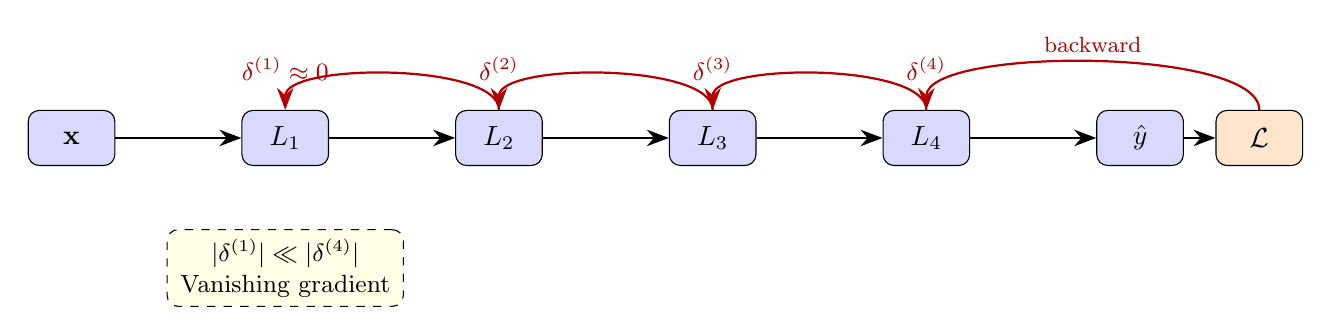
\begin{tikzpicture}[
      node distance=1.6cm,
      layer/.style={draw,rounded corners,minimum width=1.1cm,
                    minimum height=0.7cm,fill=blue!15},
      arrow/.style={-{Stealth[scale=1.2]},thick},
      gradarrow/.style={-{Stealth[scale=1.2]},thick,red!70!black},
    ]
    % Forward pass nodes
    \node[layer] (x)  {$\mathbf{x}$};
    \node[layer,right=of x]  (l1) {$L_1$};
    \node[layer,right=of l1] (l2) {$L_2$};
    \node[layer,right=of l2] (l3) {$L_3$};
    \node[layer,right=of l3] (l4) {$L_4$};
    \node[layer,right=of l4] (out){$\hat{y}$};
    \node[right=0.4cm of out,draw,fill=orange!20,rounded corners,
          minimum width=1.1cm,minimum height=0.7cm] (loss) {$\loss$};

    % Forward arrows
    \foreach \s/\t in {x/l1,l1/l2,l2/l3,l3/l4,l4/out,out/loss}
      \draw[arrow] (\s) -- (\t);

    % Gradient labels (decreasing magnitude)
    \node[above=0.25cm of l4,red!70!black,font=\small] (g4) {$\delta^{(4)}$};
    \node[above=0.25cm of l3,red!70!black,font=\small] (g3) {$\delta^{(3)}$};
    \node[above=0.25cm of l2,red!70!black,font=\small] (g2) {$\delta^{(2)}$};
    \node[above=0.25cm of l1,red!70!black,font=\small] (g1) {$\delta^{(1)} \approx 0$};

    % Backward arrows
    \draw[gradarrow] (loss.north) .. controls +(0,0.8) and +(0,0.8)
          .. node[above,font=\footnotesize]{backward} (l4.north);
    \draw[gradarrow] (l4.north) .. controls +(0,0.6) and +(0,0.6) .. (l3.north);
    \draw[gradarrow] (l3.north) .. controls +(0,0.6) and +(0,0.6) .. (l2.north);
    \draw[gradarrow] (l2.north) .. controls +(0,0.6) and +(0,0.6) .. (l1.north);

    % Magnitude annotation
    \node[below=0.8cm of l1,align=center,font=\small,
          draw,dashed,rounded corners,fill=yellow!10,
          minimum width=3cm] {
      $|\delta^{(1)}| \ll |\delta^{(4)}|$\\
      Vanishing gradient
    };

  \end{tikzpicture}
  \caption{Backward gradient flow in a 4-layer sigmoid network.  The
           gradient signal $\delta^{(\ell)}$ decreases exponentially
           as it travels from the output layer toward the input.}
  \label{fig:gradient_flow}
\end{figure}

%------------------------------------------------------------------
\subsection{TikZ Diagram: Sigmoid Saturation}
\label{ssec:tikz_sigmoid}
%------------------------------------------------------------------

\cref{fig:sigmoid_deriv} shows why the sigmoid derivative is bounded
above by $0.25$, the key mathematical cause of vanishing gradients.

\begin{figure}[htbp]
  \centering
  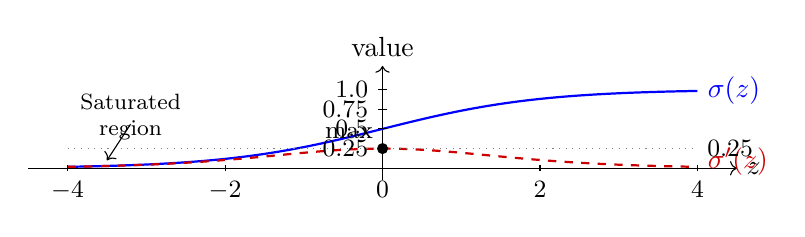
\begin{tikzpicture}[scale=1.0]
    % Axes
    \draw[->] (-4.5,0) -- (4.5,0) node[right] {$z$};
    \draw[->] (0,-0.15) -- (0,1.3) node[above] {value};

    % Sigmoid curve (piecewise linear approximation via control points)
    \draw[blue,thick,domain=-4:4,samples=100]
      plot (\x, {1/(1+exp(-\x))})
      node[right] {$\sigma(z)$};

    % Derivative curve
    \draw[red!80!black,thick,dashed,domain=-4:4,samples=100]
      plot (\x, {(1/(1+exp(-\x)))*(1-(1/(1+exp(-\x))))})
      node[right,yshift=2pt] {$\sigma'(z)$};

    % Max of derivative annotation
    \draw[gray,dotted] (-4,0.25) -- (4,0.25)
      node[right,font=\small,black] {$0.25$};
    \fill (0,0.25) circle (2pt) node[above left,font=\small] {max};

    % Saturation annotation
    \node[font=\footnotesize,align=center] at (-3.2,0.65)
      {Saturated\\region};
    \draw[->] (-3.2,0.56) -- (-3.5,0.1);

    % Ticks
    \foreach \x in {-4,-2,0,2,4}
      \draw (\x,0.04) -- (\x,-0.04) node[below,font=\small] {$\x$};
    \foreach \y in {0.25,0.5,0.75,1.0}
      \draw (0.06,\y) -- (-0.06,\y) node[left,font=\small] {$\y$};
  \end{tikzpicture}
  \caption{Sigmoid $\sigma(z)$ (solid blue) and its derivative
           $\sigma'(z)=\sigma(z)(1-\sigma(z))$ (dashed red).  The
           derivative is bounded above by $0.25$, and approaches zero
           in both saturated regions ($z \to \pm\infty$).}
  \label{fig:sigmoid_deriv}
\end{figure}

%------------------------------------------------------------------
\subsection{Mitigation Strategies}
\label{ssec:vg_mitigations}
%------------------------------------------------------------------

\begin{table}[htbp]
  \centering
  \caption{Strategies to mitigate the vanishing gradient problem.}
  \label{tab:vg_mitigations}
  \begin{tabularx}{\linewidth}{lX}
    \toprule
    \textbf{Strategy} & \textbf{Mechanism} \\
    \midrule
    ReLU activation      & Derivative is $1$ for $z > 0$; avoids
                           exponential decay \\
    Batch Normalisation  & Re-centres and re-scales activations per
                           mini-batch; reduces saturation \\
    Residual connections & Adds a skip connection $\mathbf{x} +
                           F(\mathbf{x})$; gradient can flow directly
                           through the skip path \\
    Weight initialisation & Xavier / He init ensures variance is
                            preserved across layers at the start of
                            training \\
    Gradient clipping    & Caps the gradient norm to prevent both
                           vanishing and exploding gradients \\
    LSTM / GRU gates     & Gating mechanism provides a \emph{constant
                           error carousel} for recurrent networks \\
    \bottomrule
  \end{tabularx}
\end{table}

%------------------------------------------------------------------
\subsection{Algorithm: Backpropagation with Gradient Monitoring}
\label{ssec:backprop_algo}
%------------------------------------------------------------------

\cref{alg:backprop} presents the backpropagation algorithm augmented
with a gradient-norm diagnostic step, which helps detect vanishing or
exploding gradients during training.

\begin{algorithm}[htbp]
  \DontPrintSemicolon
  \caption{Backpropagation with Gradient-Norm Monitoring}
  \label{alg:backprop}
  \KwIn{Network weights $\{W^{(\ell)}, \mathbf{b}^{(\ell)}\}_{\ell=1}^{L}$,
        input batch $(\mathbf{X}, \mathbf{Y})$,
        learning rate $\eta$, diagnostic flag \texttt{verbose}}
  \KwOut{Updated weights}
  \BlankLine
  \tcp{Forward pass}
  $\mathbf{a}^{(0)} \leftarrow \mathbf{X}$\;
  \For{$\ell = 1$ \KwTo $L$}{
    $\mathbf{z}^{(\ell)} \leftarrow W^{(\ell)}\mathbf{a}^{(\ell-1)} + \mathbf{b}^{(\ell)}$\;
    $\mathbf{a}^{(\ell)} \leftarrow f^{(\ell)}\!\left(\mathbf{z}^{(\ell)}\right)$\;
  }
  $\hat{\mathbf{Y}} \leftarrow \mathbf{a}^{(L)}$\;
  $\loss \leftarrow \frac{1}{N}\|\mathbf{Y} - \hat{\mathbf{Y}}\|^2$\;
  \BlankLine
  \tcp{Backward pass}
  $\boldsymbol{\delta}^{(L)} \leftarrow \frac{2}{N}(\hat{\mathbf{Y}} - \mathbf{Y}) \odot {f^{(L)}}'(\mathbf{z}^{(L)})$\;
  \For{$\ell = L-1$ \KwTo $1$}{
    $\boldsymbol{\delta}^{(\ell)} \leftarrow \left({W^{(\ell+1)}}^{\!\top}\boldsymbol{\delta}^{(\ell+1)}\right) \odot {f^{(\ell)}}'(\mathbf{z}^{(\ell)})$\;
    \If{\texttt{verbose}}{
      \textbf{print} $\ell$, $\|\boldsymbol{\delta}^{(\ell)}\|_2$\;
    }
  }
  \BlankLine
  \tcp{Weight update}
  \For{$\ell = 1$ \KwTo $L$}{
    $W^{(\ell)} \leftarrow W^{(\ell)} - \eta\,\boldsymbol{\delta}^{(\ell)}\,{\mathbf{a}^{(\ell-1)}}^{\!\top}$\;
    $\mathbf{b}^{(\ell)} \leftarrow \mathbf{b}^{(\ell)} - \eta\,\boldsymbol{\delta}^{(\ell)}\mathbf{1}$\;
  }
  \Return{$\{W^{(\ell)}, \mathbf{b}^{(\ell)}\}$}\;
\end{algorithm}

%==================================================================
\section{PyTorch vs.\ TensorFlow: A Framework Comparison}
\label{sec:frameworks}
%==================================================================

The quiz brought to light that students who had been taught exclusively
in PyTorch were unfamiliar with TensorFlow's eager-execution,
gradient-tape API.  This section provides the conceptual bridge.

%------------------------------------------------------------------
\subsection{Design Philosophy}
\label{ssec:design}
%------------------------------------------------------------------

\begin{keyinsight}
As Prof.\ Prasanna emphasised: \textit{``TensorFlow is maximum used for
production and PyTorch has been used for development and research
models.''  }Both frameworks implement the same mathematical operations.
The differences are primarily in API style and the execution model
(eager vs.\ graph-based compilation).
\end{keyinsight}

%------------------------------------------------------------------
\subsection{Gradient Computation: \texttt{autograd} vs.\ \texttt{GradientTape}}
\label{ssec:grad_compute}
%------------------------------------------------------------------

\paragraph{PyTorch autograd.}
\begin{verbatim}
import torch

x  = torch.tensor([[1.0, 0.0, 0.0]])
W1 = torch.randn(3, 4, requires_grad=True)
b1 = torch.zeros(4,  requires_grad=True)
W2 = torch.randn(4, 1, requires_grad=True)
b2 = torch.zeros(1,  requires_grad=True)

# Forward
z1 = x @ W1 + b1
a1 = torch.relu(z1)
z2 = a1 @ W2 + b2
loss = z2.mean()

# Backward
loss.backward()
print(W1.grad)   # dL/dW1
\end{verbatim}

\paragraph{TensorFlow 2 GradientTape.}
\begin{verbatim}
import tensorflow as tf

x  = tf.constant([[1.0, 0.0, 0.0]])
W1 = tf.Variable(tf.random.normal([3, 4]))
b1 = tf.Variable(tf.zeros([4]))
W2 = tf.Variable(tf.random.normal([4, 1]))
b2 = tf.Variable(tf.zeros([1]))

with tf.GradientTape() as tape:
    z1   = tf.matmul(x, W1) + b1
    a1   = tf.nn.relu(z1)
    z2   = tf.matmul(a1, W2) + b2
    loss = tf.reduce_mean(z2)

grads = tape.gradient(loss, [W1, b1, W2, b2])
print(grads[0])  # dL/dW1
\end{verbatim}

The key structural difference is that in PyTorch the computational
graph is built implicitly during the forward pass and
\texttt{.backward()} traverses it; in TensorFlow~2 the
\texttt{GradientTape} context manager \emph{explicitly records}
operations so that \texttt{tape.gradient} can replay them.  Conceptually
both implement \cref{eq:chain,eq:delta_L,eq:delta_l,eq:dL_dW}.

%------------------------------------------------------------------
\subsection{Architecture Diagram: PyTorch \texttt{nn.Module} MLP}
\label{ssec:tikz_nnmodule}
%------------------------------------------------------------------

\cref{fig:nnmodule} shows the component structure of a two-layer MLP
implemented with PyTorch's \texttt{nn.Module} API, which is the subject
of the slide deck referenced for Session~09
(\texttt{05-PyTorchDL-NNmodule}).

\begin{figure}[htbp]
  \centering
  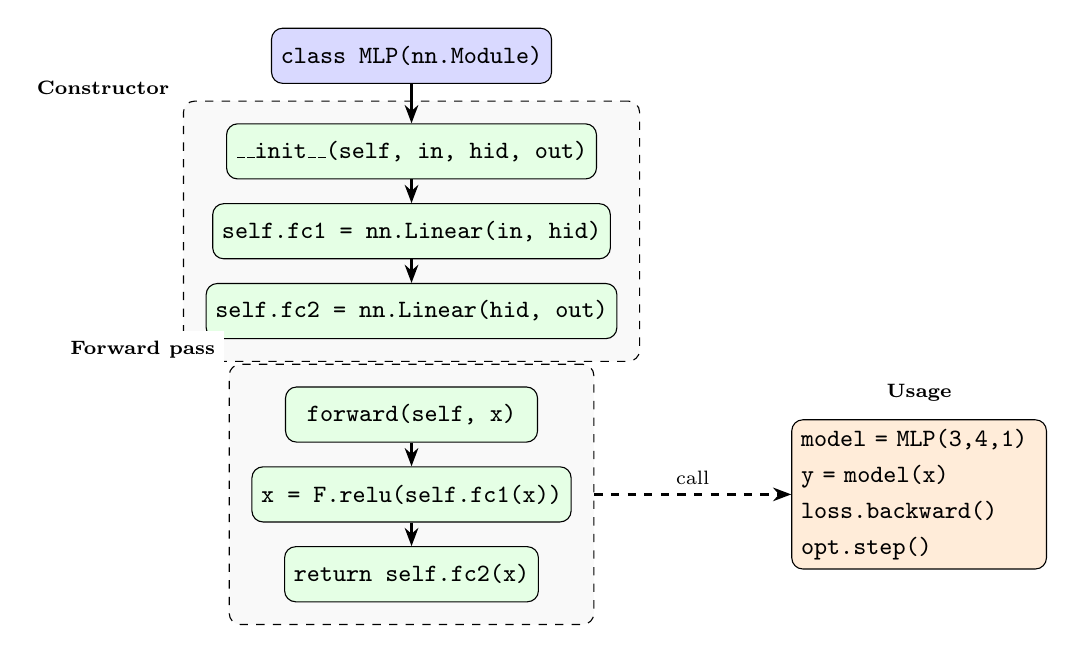
\begin{tikzpicture}[
      box/.style={draw,rounded corners,minimum width=3.2cm,
                  minimum height=0.7cm,fill=green!10,align=center,
                  font=\small},
      container/.style={draw,dashed,rounded corners,
                        fill=gray!5,inner sep=8pt},
      arrow/.style={-{Stealth},thick},
    ]

    % MLP class
    \node[box,fill=blue!15] (cls) {\texttt{class MLP(nn.Module)}};

    % __init__
    \node[box,below=0.5cm of cls] (init)
      {\texttt{\_\_init\_\_(self, in, hid, out)}};
    \node[box,below=0.3cm of init] (l1)
      {\texttt{self.fc1 = nn.Linear(in, hid)}};
    \node[box,below=0.3cm of l1]  (l2)
      {\texttt{self.fc2 = nn.Linear(hid, out)}};

    % forward
    \node[box,below=0.6cm of l2] (fwd)
      {\texttt{forward(self, x)}};
    \node[box,below=0.3cm of fwd] (r1)
      {\texttt{x = F.relu(self.fc1(x))}};
    \node[box,below=0.3cm of r1]  (r2)
      {\texttt{return self.fc2(x)}};

    % Container around __init__ block
    \begin{scope}[on background layer]
      \node[container,fit=(init)(l1)(l2)] (initbox) {};
      \node[container,fit=(fwd)(r1)(r2)]  (fwdbox)  {};
    \end{scope}
    \node[above left=-0.05cm and 0.05cm of initbox,
          font=\scriptsize,fill=white] {\textbf{Constructor}};
    \node[above left=-0.05cm and 0.05cm of fwdbox,
          font=\scriptsize,fill=white] {\textbf{Forward pass}};

    % Arrows
    \draw[arrow] (cls)  -- (init);
    \draw[arrow] (init) -- (l1);
    \draw[arrow] (l1)   -- (l2);
    \draw[arrow] (fwd)  -- (r1);
    \draw[arrow] (r1)   -- (r2);

    % Usage block
    \node[box,right=2.5cm of fwdbox,fill=orange!15,
          minimum width=3.2cm,align=left,
          text width=3cm] (usage) {%
      \texttt{model = MLP(3,4,1)}\\[2pt]
      \texttt{y = model(x)}\\[2pt]
      \texttt{loss.backward()}\\[2pt]
      \texttt{opt.step()}
    };
    \node[above=0.1cm of usage,font=\scriptsize\bfseries]
      {Usage};

    \draw[arrow,dashed] (fwdbox.east) -- (usage.west)
      node[midway,above,font=\scriptsize]{call};

  \end{tikzpicture}
  \caption{Structure of a two-layer MLP using PyTorch's
           \texttt{nn.Module} API, as covered in slide deck
           \texttt{05-PyTorchDL-NNmodule}.}
  \label{fig:nnmodule}
\end{figure}

%==================================================================
\section{Looking Ahead: CNN, RNN, LSTM, Transformer}
\label{sec:lookahead}
%==================================================================

At the conclusion of Session~09, Prof.\ Prasanna provided a brief
outlook on the remainder of the course.  His key message was:

\begin{quote}
  ``Once these fundamentals are in place -- one or two more classes on
  the \texttt{nn.Module} code -- we will enter into deep neural networks
  like CNN, RNN, LSTM, and even the transformer.  The fundamentals will
  not change much.  The architecture changes, but ultimately there will
  always be a backpropagation, and if you know how it works now, that is
  going to be the same for almost all the architectures you are going
  to study.''
\end{quote}

\cref{tab:architecture_comparison} shows how the core components of the
MLP extend to more complex architectures.

\begin{table}[htbp]
  \centering
  \caption{Extension of MLP fundamentals to advanced architectures.}
  \label{tab:architecture_comparison}
  \begin{tabularx}{\linewidth}{lXX}
    \toprule
    \textbf{Architecture} & \textbf{Key Addition over MLP}
                          & \textbf{Backprop variant} \\
    \midrule
    MLP           & Fully-connected layers only
                  & Standard backprop (\cref{alg:backprop}) \\
    CNN           & Convolutional + pooling layers; weight sharing
                  & Backprop through convolution \\
    RNN           & Recurrent hidden state; shared weights over time
                  & Backpropagation Through Time (BPTT) \\
    LSTM          & Gated memory cell; constant error carousel
                  & BPTT with vanishing-gradient mitigation \\
    Transformer   & Self-attention mechanism; no recurrence
                  & Backprop through attention weights \\
    \bottomrule
  \end{tabularx}
\end{table}

\begin{example}[Conceptual continuity from MLP to CNN]
In an MLP a hidden unit computes
$a_j = f\!\left(\sum_i w_{ji} x_i + b_j\right)$.
In a CNN a feature map at position $(r,c)$ computes
\[
  a_{rc} = f\!\!\left(\sum_{p}\sum_{q} k_{pq}\, x_{r+p,\,c+q} + b\right),
\]
where $k_{pq}$ is a \emph{shared} convolutional kernel.  The
backpropagation gradient with respect to $k_{pq}$ is simply
\[
  \frac{\partial\loss}{\partial k_{pq}}
  = \sum_{r}\sum_{c} \delta_{rc}\, x_{r+p,\,c+q},
\]
which is a cross-correlation of the error signal with the input patch --
entirely analogous to \cref{eq:dL_dW}.
\end{example}

%==================================================================
\section{Summary and Conclusion}
\label{sec:conclusion}
%==================================================================

Session~09 served as a pivotal checkpoint in the deep learning course.
The mid-course quiz assessed eight months of foundational material and
the subsequent discussion surfaced three important lessons.

\paragraph{Lesson 1 -- Read the figure, not only the concept.}
The vanishing gradient question demonstrated that exam answers must be
grounded in the \emph{specific scenario presented}, not just in the
canonical formulation.  A graph showing steeper gradients in early
layers and flat gradients in later layers inverts the classical picture;
the answer must reflect that inversion.

\paragraph{Lesson 2 -- Frameworks are wrappers, not new mathematics.}
The PyTorch/TensorFlow gap is syntactic, not mathematical.  Every
operation -- matrix multiply, gradient computation, parameter update --
maps directly to the same equation regardless of which framework
exposes it.  The ability to translate between API styles is a
professional skill, not a conceptual hurdle.

\paragraph{Lesson 3 -- Fundamentals are durable.}
As Prof.\ Prasanna emphasised, the chain rule, delta computation, and
gradient descent that underpin MLP training apply unchanged to CNN,
RNN, LSTM, and Transformer.  Investment in understanding these
fundamentals deeply pays compound interest throughout the remainder of
the course.

\medskip
\noindent
\textbf{Next session (Session~10)} resumes technical content with deep
feedforward networks and the PyTorch \texttt{nn.Module} framework in
detail.

\begin{keyinsight}
The core equations to remember from Sessions~01--09:
\begin{align}
  \text{Forward:}\quad
  \mathbf{z}^{(\ell)} &= W^{(\ell)}\mathbf{a}^{(\ell-1)} + \mathbf{b}^{(\ell)},
  \quad \mathbf{a}^{(\ell)} = f\!\left(\mathbf{z}^{(\ell)}\right), \notag \\
  \text{Backward:}\quad
  \boldsymbol{\delta}^{(\ell)} &=
    \left({W^{(\ell+1)}}^{\!\top}\boldsymbol{\delta}^{(\ell+1)}\right)
    \odot f'\!\left(\mathbf{z}^{(\ell)}\right), \notag \\
  \text{Update:}\quad
  W^{(\ell)} &\leftarrow W^{(\ell)}
    - \eta\,\boldsymbol{\delta}^{(\ell)}\,{\mathbf{a}^{(\ell-1)}}^{\!\top}. \notag
\end{align}
These three lines encode all of deep learning up to this point.
\end{keyinsight}

%------------------------------------------------------------------
\appendix
%------------------------------------------------------------------
\section{Quick Reference: Key Formulae}
\label{app:formulae}

\begin{align}
  &\text{Sigmoid:} & \sigma(z) &= \frac{1}{1+e^{-z}}, \quad
    \sigma'(z) = \sigma(z)(1-\sigma(z)) \leq 0.25, \label{eq:sig_ref}\\[4pt]
  &\text{Tanh:}    & \tanh'(z) &= 1 - \tanh^2(z) \leq 1, \label{eq:tanh_ref}\\[4pt]
  &\text{ReLU:}    & f'(z) &= \begin{cases}1 & z > 0 \\ 0 & z \leq 0\end{cases},
    \label{eq:relu_ref}\\[4pt]
  &\text{MSE:}     & \loss &= \frac{1}{N}\sum_i (y_i - \hat{y}_i)^2,
    \quad \frac{\partial\loss}{\partial\hat{y}_i} = \frac{-2}{N}(y_i - \hat{y}_i),
    \label{eq:mse_ref}\\[4pt]
  &\text{Perceptron update:} &
    w_i &\leftarrow w_i + \eta(y-\hat{y})x_i. \label{eq:perc_ref}
\end{align}

\section{PyTorch Snippet: Two-Layer MLP with Training Loop}
\label{app:pytorch}

The following complete snippet illustrates the PyTorch \texttt{nn.Module}
pattern and a basic training loop, synthesising the material assessed
in the quiz.

\begin{verbatim}
import torch
import torch.nn as nn
import torch.optim as optim

class TwoLayerMLP(nn.Module):
    def __init__(self, in_dim, hid_dim, out_dim):
        super().__init__()
        self.fc1 = nn.Linear(in_dim,  hid_dim)
        self.fc2 = nn.Linear(hid_dim, out_dim)

    def forward(self, x):
        x = torch.relu(self.fc1(x))
        return self.fc2(x)

# Instantiate
model = TwoLayerMLP(3, 8, 1)
criterion = nn.MSELoss()
optimizer = optim.SGD(model.parameters(), lr=0.01)

# Training loop
for epoch in range(100):
    optimizer.zero_grad()          # clear gradients
    y_hat = model(X_train)         # forward pass
    loss  = criterion(y_hat, y_train)
    loss.backward()                # backprop
    optimizer.step()               # update weights

    # Gradient norm monitoring (for vanishing gradient detection)
    for name, param in model.named_parameters():
        if param.grad is not None:
            print(f"{name}: grad norm = {param.grad.norm():.4f}")
\end{verbatim}

\end{document}
